\documentclass[11pt]{article}

\usepackage[margin=1in]{geometry}
\usepackage{fontenc}
\usepackage{inputenc}
\usepackage[pdftex,colorlinks,linkcolor=blue,citecolor=OliveGreen,urlcolor=blue,filecolor=blue]{hyperref}
\usepackage{enumitem}
\usepackage{titlesec}
\usepackage{parskip}
\usepackage[dvipsnames]{xcolor}
\usepackage{booktabs}
\usepackage[numbers]{natbib}

\usepackage{amsmath,amsthm,amssymb}
\usepackage{graphicx}
\usepackage{array}
\usepackage{pifont}
\usepackage{tikz}
\usetikzlibrary{arrows.meta,positioning,fit,backgrounds,calc,shapes.geometric,decorations.pathreplacing,patterns}

% ---- figure style ----
\definecolor{c1mem}{HTML}{2C6E9B}   % type 1 memory
\definecolor{c2mem}{HTML}{9B5B2C}   % type 2 memory
\definecolor{cplan}{HTML}{3E7A4E}   % planning / execution
\definecolor{cenv}{HTML}{555555}    % environment
\definecolor{cbg1}{HTML}{E8F0F6}
\definecolor{cbg2}{HTML}{F6EEE6}
\definecolor{cbgp}{HTML}{EAF2EC}
\definecolor{cbge}{HTML}{EFEFEF}

\tikzset{
  blk/.style={draw,rounded corners=2pt,align=center,inner sep=3.5pt,font=\scriptsize},
  mem1/.style={blk,draw=c1mem,fill=cbg1},
  mem2/.style={blk,draw=c2mem,fill=cbg2},
  plan/.style={blk,draw=cplan,fill=cbgp},
  env/.style={blk,draw=cenv,fill=cbge},
  flow/.style={-{Latex[length=1.6mm]},thick},
  rd/.style={-{Latex[length=1.6mm]},draw=c2mem,dashed,thin},
  rd1/.style={-{Latex[length=1.6mm]},draw=c1mem,dashed,thin},
  lbl/.style={font=\scriptsize\itshape,inner sep=1.5pt},
  slbl/.style={font=\tiny,inner sep=1pt},
}

% ---- notation ----
\newcommand{\llm}[1]{\mathrm{LLM}_{\mathrm{#1}}}
\newcommand{\calS}{\mathcal{S}}
\newcommand{\calA}{\mathcal{A}}
\newcommand{\calO}{\mathcal{O}}
\newcommand{\calF}{\mathcal{F}}
\newcommand{\calV}{\mathcal{V}}
\newcommand{\calM}{\mathcal{M}}
\newcommand{\calE}{\mathcal{E}}
\newcommand{\calB}{\mathcal{B}}
\newcommand{\calQ}{\mathcal{Q}}
\newcommand{\calK}{\mathcal{K}}
\newcommand{\calX}{\mathcal{X}}
\newcommand{\Rel}{R}
\newcommand{\shat}{\hat{s}}
\newcommand{\sA}{s^{\mathrm{A}}}
\newcommand{\sP}{s^{\mathrm{P}}}
\newcommand{\sM}{s^{\mathrm{M}}}
\newcommand{\FA}{\calF^{\mathrm{A}}}
\newcommand{\FP}{\calF^{\mathrm{P}}}
\newcommand{\FM}{\calF^{\mathrm{M}}}
\newcommand{\Read}{\mathrm{Read}}
\newcommand{\Write}{\mathrm{Write}}
\newcommand{\Trace}{\mathrm{Trace}}
\newcommand{\loc}{\mathrm{loc}}
\newcommand{\prov}{\mathrm{prov}}
\newcommand{\vol}{\mathrm{vol}}
\newcommand{\stat}{\mathrm{status}}
\newcommand{\attr}{\mathrm{attr}}
\newcommand{\dist}{\mathrm{dist}}
\newcommand{\type}{\mathrm{type}}
\newcommand{\tobs}{t_{\mathrm{obs}}}

% lifecycle tables
\newenvironment{lifecycle}{\begin{center}\small\begin{tabular}{@{}>{\raggedright\arraybackslash}p{0.17\textwidth}>{\raggedright\arraybackslash}p{0.36\textwidth}>{\raggedright\arraybackslash}p{0.40\textwidth}@{}}\toprule Field & Set at creation & Later changes \\ \midrule}{\bottomrule\end{tabular}\end{center}}

% circled letter tags used in figures
\newcommand{\circledtag}[1]{\tikz[baseline=(ct.base)]{\node[draw,circle,inner sep=0.8pt,minimum size=2.6mm,line width=0.35pt,font=\tiny] (ct) {#1};}}

% float placement
\renewcommand{\topfraction}{0.92}
\renewcommand{\bottomfraction}{0.75}
\renewcommand{\textfraction}{0.06}
\renewcommand{\floatpagefraction}{0.75}
\setcounter{topnumber}{2}
\setcounter{totalnumber}{3}

\begin{document}

\section{Problem Setup}
\label{sec:setup}

This section formalizes the decision-making problem, fixes the representation of states and observations for the video-game setting, and defines the task structure under which memory is evaluated.

\subsection{Decision making under partial observability}
\label{sec:pomdp}

\paragraph{POMDPs.}
The task faced by the agent is a partially observable Markov decision process (POMDP) $(\calS, \calA, \calO, p, Z, r)$, where $\calS$ is the set of world states, $\calA$ the set of primitive actions, $\calO$ the set of observations, $p:\calS\times\calA\to\Delta(\calS)$ the transition function, $Z:\calS\to\Delta(\calO)$ the observation function, and $r:\calS\times\calA\to\mathbb{R}$ the reward function. Concretely, $\calA$ is the set of \emph{control primitives} of the environment: the low-level API calls through which the agent acts on the world (navigate to a location, interact with an element, use a possession), and which in our system are issued by generated code. At each discrete time step $t=0,1,\dots$, the environment is in state $s_t\in\calS$, the agent receives an observation $o_t\sim Z(\cdot\mid s_t)$, and chooses an action $a_t\in\calA$; the next state is sampled as $s_{t+1}\sim p(\cdot\mid s_t,a_t)$. The agent does not observe $s_t$. Its information at time $t$ is the history $h_t := (o_0,a_0,o_1,\dots,a_{t-1},o_t)$, and a policy is a mapping $\pi: h_t\mapsto \Delta(\calA)$. The agent aims to maximize the expected cumulative discounted reward $\mathbb{E}_\pi[\sum_{t\ge 0}\gamma^t r(s_t,a_t)]$ with discount $\gamma\in[0,1)$. In the tasks considered here, $r$ is sparse: it is the indicator of a task-specific success predicate, defined in Section~\ref{sec:tasks}.

Because the policy must condition on $h_t$ rather than $s_t$, and $h_t$ grows without bound, the agent maintains a finite \emph{state estimate} $\shat_t$ that summarizes $h_t$ for the purpose of decision making. The construction and maintenance of $\shat_t$ is the role of the state memory developed in Section~\ref{sec:type1}.

\paragraph{Temporal abstraction.}
An option $\omega\in\Omega$ is a pair $(\pi_\omega,\beta_\omega)$ of an in-option policy $\pi_\omega:h_t\mapsto\Delta(\calA)$ and a termination function $\beta_\omega:h_t\mapsto\{0,1\}$. Options are executed in the call-and-return manner: the agent follows $\pi_\omega$ until $\beta_\omega=1$, then selects the next option. An episode therefore decomposes into a sequence of option segments delimited by boundary times $0=t_0<t_1<\dots$, where option $\omega_i$ executes over steps $[t_{i-1},t_i)$ and terminates at $t_i$. We index quantities by \emph{option index} $i$ when they are defined at option boundaries, and by \emph{time step} $t$ when they are defined at every step.

Options are represented as natural-language strings rather than abstract symbols. Consequently, $\pi_\omega$ and $\beta_\omega$ are not given a priori; they are realized on the fly by prompting a large language model (LLM) to synthesize executable code and termination predicates from the string $\omega$ and the current state estimate (Section~\ref{sec:type1-plan}).

\paragraph{LLM prompting.}
Let $\mathrm{LLM}(y\mid x)$ denote the probability that an LLM outputs token sequence $y$ given input $x$. We write $\llm{name}(y\mid x)=\mathrm{LLM}(y\mid \mathrm{prompt}_{\mathrm{name}}(x))$ for the practice of wrapping the input with a fixed prompt template specific to the module $\mathrm{name}$. All modules in this proposal are of this form; no model parameters are updated.

\subsection{States, observations, and terminology for the video-game setting}
\label{sec:states}

\paragraph{Structured states.}
We represent states and state estimates as structured key-value records. Let $\calF$ be a universe of typed \emph{feature paths} (e.g., \texttt{agent.possessions.wood}, \texttt{percept.entities.cow}) with value domains $\calV$. A (partial) state record is a partial assignment $\shat:\calF\rightharpoonup\calV$, and $\shat|_{F}$ denotes its restriction to $F\subseteq\calF$. The universe is partitioned into three components:
\begin{itemize}[leftmargin=1.5em,itemsep=1pt]
\item $\FA$, the \emph{agent state}: what the agent possesses and its own condition (possessions, held tools, health, pose). These features are exposed in every observation.
\item $\FP$, the \emph{perceptual field}: elements of the world that are currently perceivable by the agent (entities, resources, and terrain within sensing range). These features are exposed in the observation but are transient: an element leaves $\FP$ as soon as it leaves sensing range.
\item $\FM$, the \emph{remembered world}: elements of the world that were perceived earlier and are no longer in the perceptual field, together with elements asserted by the task description. These features are never exposed in an observation; they exist in $\shat_t$ only if maintained by memory.
\end{itemize}
Accordingly, an observation is a record over the first two components, $o_t:\FA\cup\FP\rightharpoonup\calV$, whereas the true state $s_t$ additionally contains all world elements outside the perceptual field.
A state estimate is a record
\begin{equation}
\shat_t=(\sA_t,\sP_t,\sM_t),\qquad \sA_t=o_t|_{\FA},\quad \sP_t=o_t|_{\FP},\quad \sM_t=\Read(\calM_t,\cdot),
\label{eq:state-estimate}
\end{equation}
where the first two components are copied from the current observation and the third is read from a memory store $\calM_t$ (Section~\ref{sec:type1}). 


\begin{figure}[t]
\centering
% Spatial partial observability: map with sensing range, and the three-component state record.
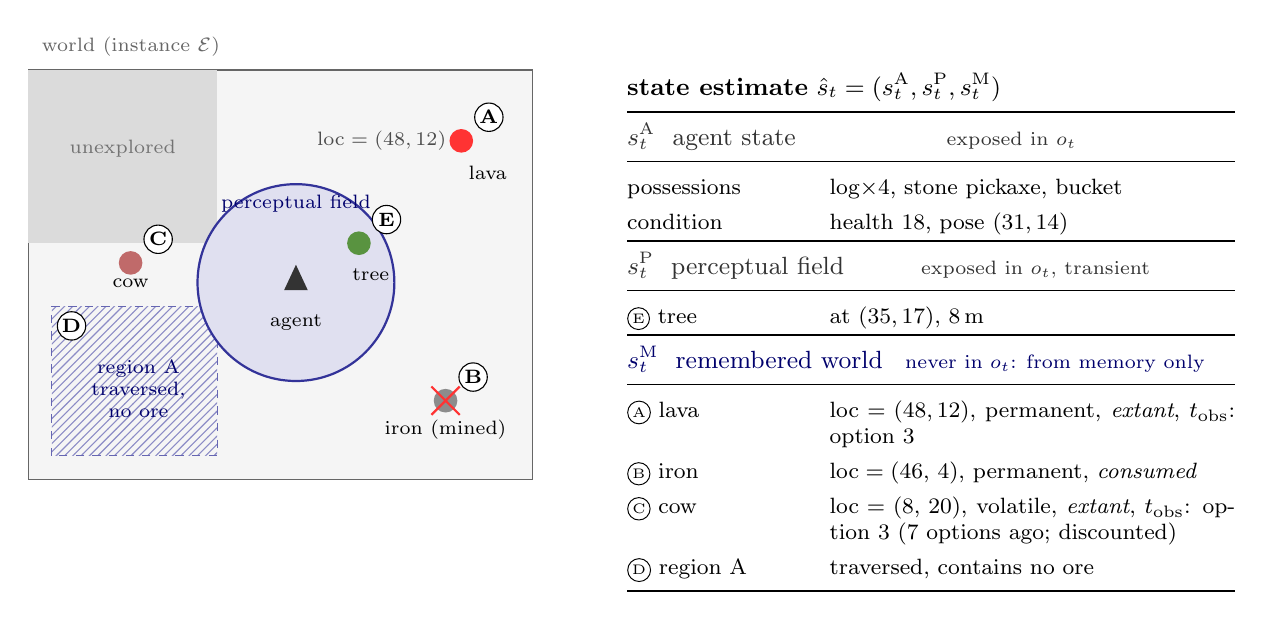
\begin{tikzpicture}[
  font=\small,
  el/.style={circle, inner sep=0pt, minimum size=3mm},
  lab/.style={font=\scriptsize, align=left, inner sep=1pt},
  tag/.style={circle, draw, inner sep=0.6pt, font=\scriptsize\bfseries, fill=white, minimum size=3.6mm},
]
% ---------- map ----------
\begin{scope}
  % world
  \fill[black!4] (0,0) rectangle (6.4,5.2);
  \draw[black!60] (0,0) rectangle (6.4,5.2);
  \node[anchor=south west, font=\scriptsize, black!60] at (0.05,5.25) {world (instance $\calE$)};
  % unexplored fog
  \fill[black!14] (0,3.0) rectangle (2.4,5.2);
  \node[font=\scriptsize, black!55, align=center] at (1.2,4.2) {unexplored};
  % explored region A, no ore
  \fill[pattern=north east lines, pattern color=NavyBlue!45] (0.3,0.3) rectangle (2.4,2.2);
  \draw[NavyBlue!60, dashed] (0.3,0.3) rectangle (2.4,2.2);
  \node[tag] (tD) at (0.55,1.95) {D};
  \node[font=\scriptsize, NavyBlue!85!black, align=center] at (1.4,1.15) {region A\\traversed,\\no ore};
  % agent and sensing range
  \fill[NavyBlue!12] (3.4,2.5) circle (1.25);
  \draw[NavyBlue!80, thick] (3.4,2.5) circle (1.25);
  \node[font=\scriptsize, NavyBlue!85!black] at (3.4,3.5) {perceptual field};
  \node[isosceles triangle, isosceles triangle apex angle=50, fill=black!80, inner sep=0pt, minimum size=3mm, rotate=90] at (3.4,2.5) {};
  \node[font=\scriptsize] at (3.4,2.0) {agent};
  % tree inside sensing range
  \node[el, fill=OliveGreen!80] (tree) at (4.2,3.0) {};
  \node[tag] at (4.55,3.3) {E};
  \node[lab] at (4.35,2.6) {tree};
  % lava outside
  \node[el, fill=Red!80] (lava) at (5.5,4.3) {};
  \node[tag] at (5.85,4.6) {A};
  \node[lab, anchor=west] at (5.55,3.9) {lava};
  \node[lab, anchor=east, black!70] at (5.35,4.3) {$\loc=(48,12)$};
  % iron consumed
  \node[el, fill=black!45] (iron) at (5.3,1.0) {};
  \draw[Red!80, thick] (5.12,0.82) -- (5.48,1.18) (5.12,1.18) -- (5.48,0.82);
  \node[tag] at (5.65,1.3) {B};
  \node[lab, anchor=north] at (5.3,0.8) {iron (mined)};
  % cow, volatile, seen long ago
  \node[el, fill=Brown!70] (cow) at (1.3,2.75) {};
  \node[tag] at (1.65,3.05) {C};
  \node[lab, anchor=north] at (1.3,2.58) {cow};
  % observation boundary note
\end{scope}

% ---------- record ----------
\begin{scope}[shift={(7.6,0)}]
  \node[anchor=north west, inner sep=0pt] at (0,5.2) {%
  \renewcommand{\arraystretch}{1.15}%
  \begin{tabular}{@{}p{2.15cm}p{5.15cm}@{}}
  \multicolumn{2}{@{}l}{\textbf{state estimate} $\shat_t=(\sA_t,\sP_t,\sM_t)$}\\[2pt]
  \toprule
  \multicolumn{2}{@{}l}{\color{black!80}$\sA_t$ \ agent state \hfill {\scriptsize exposed in $o_t$}}\\
  \midrule
  \footnotesize possessions & \footnotesize log$\times$4, stone pickaxe, bucket\\
  \footnotesize condition & \footnotesize health 18, pose $(31,14)$\\
  \toprule
  \multicolumn{2}{@{}l}{\color{black!80}$\sP_t$ \ perceptual field \hfill {\scriptsize exposed in $o_t$, transient}}\\
  \midrule
  \footnotesize \circledtag{E} tree & \footnotesize at $(35,17)$, 8\,m\\
  \toprule
  \multicolumn{2}{@{}l}{\color{NavyBlue!85!black}$\sM_t$ \ remembered world \hfill {\scriptsize never in $o_t$: from memory only}}\\
  \midrule
  \footnotesize \circledtag{A} lava & \footnotesize $\loc=(48,12)$, permanent, \emph{extant}, $\tobs$: option 3\\
  \footnotesize \circledtag{B} iron & \footnotesize $\loc=(46,\,4)$, permanent, \emph{consumed}\\
  \footnotesize \circledtag{C} cow & \footnotesize $\loc=(8,\,20)$, volatile, \emph{extant}, $\tobs$: option 3 (7 options ago; discounted)\\
  \footnotesize \circledtag{D} region A & \footnotesize traversed, contains no ore\\
  \bottomrule
  \end{tabular}};
\end{scope}
\end{tikzpicture}

\caption{Spatial partial observability and the three-component state estimate. Left: the world is larger than the agent's sensing range. Elements inside the range (E) are in the perceptual field; elements seen earlier (A--C) and regions already traversed (D) are outside it and persist, change, or disappear unobserved. Right: the observation $o_t$ exposes only the agent state and the perceptual field; the remembered component $\sM_t$ exists only if maintained by memory, and it is what allows an option such as ``return to the lava and fill the bucket'' to be planned and executed.}
\label{fig:pomdp}
\end{figure}


\paragraph{Terminology.}
We use the following terms for the video-game setting, chosen to be domain-neutral.
\begin{itemize}[leftmargin=1.5em,itemsep=1pt]
\item An \emph{element} is any world entity the agent can refer to: an object, a resource deposit, a creature, a structure, or a spatial \emph{region}. Elements have a \emph{type}, attributes, and a location.
\item A \emph{locator} $\loc(\cdot)$ is the information an option needs to re-access an element: coordinates in a 3D world, a room in a building, a path or address in a software environment. Locators are the bridge between remembered elements and executable options, since the control primitives of $\calA$ navigate by locator.
\end{itemize}
In this and the following section, observations are structured records provided by the environment API. The extension to raw video observations, where $\sA_t$ and $\sP_t$ must themselves be inferred from pixels, is deferred to a later section; the state representation above is designed so that this extension changes only how $o_t$ is produced, not how it is consumed.

\subsection{Task structure}
\label{sec:tasks}

\paragraph{Task, instance, and goal.}
A task is a triple $(g,\calE,s_0)$: a natural-language goal $g$ with a success predicate $\mathrm{succ}_g:\calS\to\{0,1\}$ evaluated by the environment on the true state; an \emph{environment instance} $\calE$, a concrete world (in a procedurally generated game, a seed and the content generated from it); and an initial state $s_0$. Since the three are fixed together, we use \emph{task}, \emph{instance}, and \emph{goal} as synonyms and denote the task by $g$.

\paragraph{Episodes.}
The agent executes $K$ episodes of the task in sequence. Episode $k$ starts from $s_0$ in $\calE$ and runs until $\mathrm{succ}_g(s_t)=1$ or a budget is exhausted; it is scored by whether the success predicate was met. Every episode is executed in the same instance from the same initial state. Consequently, a world element found at a locator in episode $k$ exists at that locator in episode $k+1$ unless the agent consumed it, and element-level knowledge (as opposed to knowledge about element types) is transferable across episodes. This persistence is assumed throughout.


\section{State Memory: Estimation over Options}
\label{sec:type1}

\begin{figure}[tb]
\centering
\resizebox{\textwidth}{!}{% System overview: state memory (Type 1), experience memory (Type 2), planner, executor, monitor.
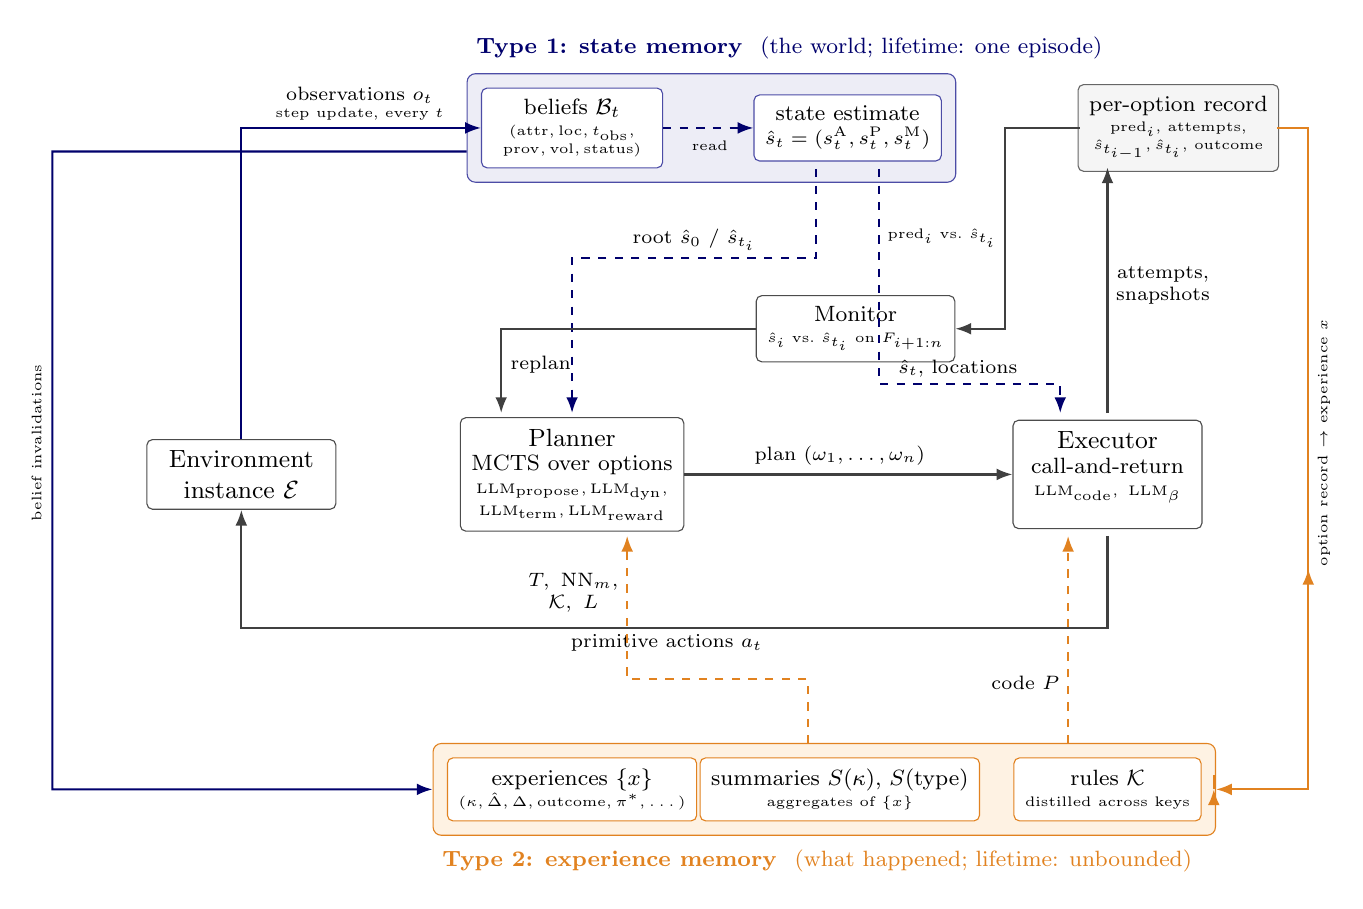
\begin{tikzpicture}[
  font=\small,
  box/.style={draw, rounded corners=2pt, align=center, inner sep=4pt, minimum height=8mm},
  core/.style={box, fill=white, draw=black!70, minimum width=24mm},
  sub1/.style={box, fill=white, draw=NavyBlue!70, minimum width=23mm, font=\footnotesize},
  sub2/.style={box, fill=white, draw=BurntOrange!90!black, minimum width=23mm, font=\footnotesize},
  band1/.style={draw=NavyBlue!70, fill=NavyBlue!7, rounded corners=3pt, inner sep=5pt},
  band2/.style={draw=BurntOrange!90!black, fill=BurntOrange!9, rounded corners=3pt, inner sep=5pt},
  flow/.style={-{Latex[length=2mm]}, thick, black!75},
  w1/.style={-{Latex[length=2mm]}, thick, NavyBlue!85!black},
  w2/.style={-{Latex[length=2mm]}, thick, BurntOrange!90!black},
  r1/.style={-{Latex[length=2mm]}, thick, NavyBlue!85!black, dashed},
  r2/.style={-{Latex[length=2mm]}, thick, BurntOrange!90!black, dashed},
  lbl/.style={font=\scriptsize, inner sep=1.5pt, align=center},
  tlab/.style={font=\tiny, inner sep=1.5pt, align=center},
]

% ================= middle row =================
\node[core] (env)  at (0,0)    {Environment\\instance $\calE$};
\node[core] (plan) at (4.2,0)  {Planner\\[-2pt]{\footnotesize MCTS over options}\\[-3pt]{\tiny $\llm{propose},\llm{dyn},$}\\[-3pt]{\tiny $\llm{term},\llm{reward}$}};
\node[core] (exec) at (11.0,0) {Executor\\[-2pt]{\footnotesize call-and-return}\\[-3pt]{\tiny $\llm{code},\ \llm{\beta}$}\\[-3pt]{\tiny\phantom{x}}};
\node[box, fill=white, draw=black!70, font=\footnotesize, minimum width=23mm] (mon) at (7.8,1.85)
  {Monitor\\[-2pt]{\tiny $\shat_i$ vs.\ $\shat_{t_i}$ on $F_{i+1:n}$}};

% ================= top band: Type 1 =================
\node[sub1] (bel) at (4.2,4.4) {beliefs $\calB_t$\\[-2pt]{\tiny $(\attr,\loc,\tobs,$}\\[-3pt]{\tiny $\prov,\vol,\stat)$}};
\node[sub1] (est) at (7.7,4.4) {state estimate\\[-1pt]{\scriptsize $\shat_t=(\sA_t,\sP_t,\sM_t)$}};
\begin{scope}[on background layer]
  \node[band1, fit=(bel)(est)] (band1) {};
\end{scope}
\node[NavyBlue!85!black, font=\footnotesize\bfseries, anchor=west] at ([yshift=3.2mm]band1.north west)
  {Type 1: state memory\ \ {\normalfont\footnotesize (the world; lifetime: one episode)}};

% per-option record, outside both memories
\node[box, fill=black!4, draw=black!60, font=\footnotesize, minimum width=25mm] (trc) at (11.9,4.4)
  {per-option record\\[-2pt]{\tiny $\mathrm{pred}_i$, attempts,}\\[-3pt]{\tiny $\shat_{t_{i-1}},\shat_{t_i}$, outcome}};

% ================= bottom band: Type 2 =================
\node[sub2] (xp)   at (4.2,-4.0)  {experiences $\{x\}$\\[-2pt]{\tiny $(\kappa,\hat\Delta,\Delta,\mathrm{outcome},\pi^\ast,\dots)$}};
\node[sub2] (stat) at (7.6,-4.0)  {summaries $S(\kappa)$, $S(\mathrm{type})$\\[-2pt]{\tiny aggregates of $\{x\}$}};
\node[sub2] (lib)  at (11.0,-4.0) {rules $\calK$\\[-2pt]{\tiny distilled across keys}};
\begin{scope}[on background layer]
  \node[band2, fit=(xp)(stat)(lib)] (band2) {};
\end{scope}
\node[BurntOrange!90!black, font=\footnotesize\bfseries, anchor=west] at ([yshift=-3.2mm]band2.south west)
  {Type 2: experience memory\ \ {\normalfont\footnotesize (what happened; lifetime: unbounded)}};

% ================= environment / executor loop =================
\draw[flow] (11.0,-0.78) -- (11.0,-1.95) -- (0,-1.95) -- (env.south);
\node[lbl, below] at (5.4,-1.97) {primitive actions $a_t$};

\draw[w1] (env.north) -- (0,4.4) -- (bel.west);
\node[lbl, above, align=center] at (1.5,4.44) {observations $o_t$\\[-2pt]{\tiny step update, every $t$}};

% ================= Type 1 internal =================
\draw[r1] (bel) -- (est);
\node[tlab, below] at (5.95,4.3) {read};

% ================= Type 1 -> planner / executor =================
\draw[r1] (7.3,3.88) -- (7.3,2.75) -- (4.2,2.75) -- (4.2,0.78);
\node[lbl, above] at (5.75,2.78) {root $\shat_0$ / $\shat_{t_i}$};

\draw[r1] (8.1,3.88) -- (8.1,1.15) -- (10.4,1.15) -- (10.4,0.78);
\node[lbl, above] at (9.1,1.18) {$\shat_t$, locations};

% ================= planner -> executor; record -> monitor -> planner =================
\draw[flow] (plan) -- (exec);
\node[lbl, above] at (7.6,0.06) {plan $(\omega_1,\dots,\omega_n)$};

\draw[flow] (11.0,0.78) -- (11.0,3.9);
\node[lbl, right, align=center] at (11.05,2.4) {attempts,\\snapshots};

\draw[flow] (10.65,4.4) -- (9.7,4.4) -- (9.7,1.85) -- (mon.east);
\node[tlab, left] at (9.65,3.0) {$\mathrm{pred}_i$ vs.\ $\shat_{t_i}$};

\draw[flow] (mon.west) -- (3.3,1.85) -- (3.3,0.78);
\node[lbl, right] at (3.36,1.4) {replan};

% ================= Type 2 reads =================
\draw[r2] (7.2,-3.42) -- (7.2,-2.6) -- (4.9,-2.6) -- (4.9,-0.78);
\node[lbl, left] at (4.85,-1.5) {$T,\ \mathrm{NN}_m,$\\$\calK,\ L$};

\draw[r2] (10.5,-3.42) -- (10.5,-0.78);
\node[lbl, left] at (10.45,-2.65) {code $P$};

% ================= cross-memory channels =================
\draw[w1] ([yshift=-3mm]band1.west) -- (-2.4,4.1) -- (-2.4,-4.0) -- (band2.west);
\node[tlab, rotate=90] at (-2.6,0.4) {belief invalidations};
\draw[w2] (13.15,4.4) -- (13.55,4.4) -- (13.55,-4.0) -- (band2.east);
\node[tlab, rotate=90] at (13.75,0.4) {option record $\to$ experience $x$};
\draw[w2] (12.35,-4.0) -- (12.35,-4.0);
\draw[w2] (13.55,-1.2) -- (13.55,-1.2);
\end{tikzpicture}
}
\caption{System overview. An option-level planner (MCTS whose modules are LLM prompts) and a call-and-return executor (LLM-generated code) are wrapped by two memories. Type 1 (top) is a recursive filter over beliefs: the step update folds every observation into the belief set, which supplies the third component $\sM_t$ of every state estimate. The option trace (right) belongs to neither memory---nothing in Type 1 reads it---but records, per option, what the planner predicted and what execution did; it feeds the monitor and, once closed, becomes an experience. Type 2 (bottom) keys those experiences by signature and is read into every prompt of the planner and executor, including at replanning calls within the same episode. Solid arrows are writes and control flow; dashed arrows are reads.}
\label{fig:overview}
\end{figure}

This section develops the memory that maintains the state estimate $\shat_t$ (\emph{Type 1 memory}; Figure~\ref{fig:overview}, top). It remembers the world: its contents are claims about world elements, and its lifetime is one episode, since the true state of a persistent instance is reset to $s_0$ at every episode start. Section~\ref{sec:type1-est} defines the memory and the operations by which it performs state estimation at the level of options. Section~\ref{sec:type1-plan} describes how planning and execution are performed on the maintained state estimate. Section~\ref{sec:type1-replan} describes replanning, which the maintained estimate makes possible.

\subsection{Option-level state estimation}
\label{sec:type1-est}
\begin{figure}[t]
\centering
% Two-rate belief filter: per-step rule updates and per-option LLM consolidation.
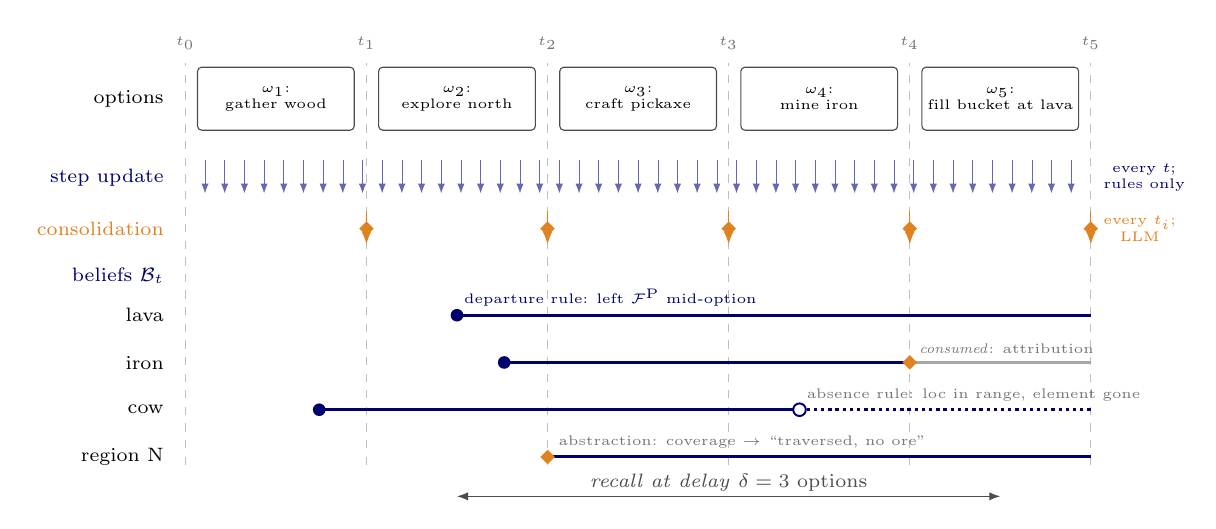
\begin{tikzpicture}[
  font=\small,
  lab/.style={font=\scriptsize, inner sep=1.5pt},
  tlab/.style={font=\tiny, inner sep=1pt, align=center},
  lane/.style={font=\scriptsize, anchor=east},
  opt/.style={draw=black!70, fill=white, rounded corners=1.5pt, minimum height=8mm, font=\tiny, inner sep=2pt, align=center, text width=1.85cm},
  ext/.style={NavyBlue!85!black, line width=1.1pt},
  unk/.style={NavyBlue!85!black, line width=1.1pt, dash pattern=on 1.2pt off 1.4pt},
  con/.style={black!35, line width=1.1pt},
  stp/.style={-{Latex[length=1.2mm]}, NavyBlue!60, very thin},
  cns/.style={-{Latex[length=1.6mm]}, BurntOrange!90!black, thin},
  ev/.style={circle, fill=NavyBlue!85!black, inner sep=0pt, minimum size=1.6mm},
  evo/.style={circle, draw=NavyBlue!85!black, fill=white, inner sep=0pt, minimum size=1.6mm, line width=0.7pt},
  evc/.style={diamond, fill=BurntOrange!90!black, inner sep=0pt, minimum size=1.9mm},
]
\def\xa{2.0}\def\xb{4.3}\def\xc{6.6}\def\xd{8.9}\def\xe{11.2}\def\xf{13.5}

% ---------- option lane ----------
\node[lane] at (\xa-0.15,5.5) {options};
\node[opt] at ({(\xa+\xb)/2},5.5) {$\omega_1$:\\gather wood};
\node[opt] at ({(\xb+\xc)/2},5.5) {$\omega_2$:\\explore north};
\node[opt] at ({(\xc+\xd)/2},5.5) {$\omega_3$:\\craft pickaxe};
\node[opt] at ({(\xd+\xe)/2},5.5) {$\omega_4$:\\mine iron};
\node[opt] at ({(\xe+\xf)/2},5.5) {$\omega_5$:\\fill bucket at lava};

\foreach \x/\n in {\xa/0,\xb/1,\xc/2,\xd/3,\xe/4,\xf/5}{
  \draw[black!25, dashed] (\x,0.85) -- (\x,5.95);
  \node[font=\tiny, black!55, anchor=south] at (\x,6.0) {$t_{\n}$};
}

% ---------- rate lanes ----------
\node[lane, NavyBlue!85!black] at (\xa-0.15,4.5) {step update};
\foreach \x in {2.25,2.5,...,13.35}{ \draw[stp] (\x,4.72) -- (\x,4.3); }
\node[tlab, NavyBlue!85!black, anchor=west] at (\xf+0.12,4.5) {every $t$;\\rules only};

\node[lane, BurntOrange!90!black] at (\xa-0.15,3.85) {consolidation};
\foreach \x in {\xb,\xc,\xd,\xe,\xf}{ \node[evc] at (\x,3.85) {}; \draw[cns] (\x,4.07) -- (\x,3.65); }
\node[tlab, BurntOrange!90!black, anchor=west] at (\xf+0.12,3.85) {every $t_i$;\\LLM};

% ---------- belief lanes ----------
\node[font=\scriptsize, anchor=east, NavyBlue!85!black] at (\xa-0.15,3.25) {beliefs $\calB_t$};
\node[lane] at (\xa-0.15,2.75) {lava};
\node[lane] at (\xa-0.15,2.15) {iron};
\node[lane] at (\xa-0.15,1.55) {cow};
\node[lane] at (\xa-0.15,0.95) {region N};

% lava: created mid-omega2 by the departure rule
\draw[ext] (5.45,2.75) -- (\xf,2.75);
\node[ev] at (5.45,2.75) {};
\node[tlab, anchor=south west, NavyBlue!85!black] at (5.5,2.82) {departure rule: left $\FP$ mid-option};

% iron: created at t2 by departure, consumed by consolidation at t4
\draw[ext] (\xc-0.55,2.15) -- (\xe,2.15);
\draw[con] (\xe,2.15) -- (\xf,2.15);
\node[ev] at (\xc-0.55,2.15) {};
\node[evc] at (\xe,2.15) {};
\node[tlab, anchor=south west, black!55] at (\xe+0.08,2.22) {\emph{consumed}: attribution};

% cow: created in omega1, unknown mid-omega4 by absence rule
\draw[ext] (3.7,1.55) -- (9.8,1.55);
\draw[unk] (9.8,1.55) -- (\xf,1.55);
\node[ev] at (3.7,1.55) {};
\node[evo] at (9.8,1.55) {};
\node[tlab, anchor=south west, black!55] at (9.85,1.62) {absence rule: $\loc$ in range, element gone};

% region N: abstracted by consolidation at t2
\draw[ext] (\xc,0.95) -- (\xf,0.95);
\node[evc] at (\xc,0.95) {};
\node[tlab, anchor=south west, black!55] at (\xc+0.1,1.02) {abstraction: coverage $\to$ ``traversed, no ore''};

% ---------- legend / recall ----------
\draw[{Latex[length=1.4mm]}-{Latex[length=1.4mm]}, black!70] (5.45,0.45) -- (12.35,0.45);
\node[lab, anchor=south, black!70, fill=white, inner sep=1.5pt] at ({(5.45+12.35)/2},0.46)
  {\emph{recall at delay} $\delta=3$ options};
\end{tikzpicture}

\caption{The belief filter at its two rates. At every time step a rule-based update (\ref{eq:step}) folds the observation into the belief set: an element leaving the perceptual field becomes a belief, a re-observed element refreshes one, and a belief whose locator is in range with the element absent becomes \emph{unknown}. At every option termination an LLM consolidation (\ref{eq:consol}) performs what rules cannot: attributing consumption to the option that caused it, and abstracting accumulated coverage into region beliefs with negative content. Line style shows belief status: solid \emph{extant}, dashed \emph{unknown}, grey \emph{consumed}. Because the update is recursive, no observation history is retained, yet the lava locator written during $\omega_2$ is still available to execute $\omega_5$ three options later.}
\label{fig:estimation}
\end{figure}


The state estimate is maintained by a recursive filter over \emph{beliefs}, claims about world elements outside the perceptual field, which constitute the remembered component $\sM_t$ of (\ref{eq:state-estimate}). The filter runs at two rates. At every time step, a rule-based update folds the current observation into the belief set; this is what makes $\sM_t$ a summary of the history $h_t$ rather than a record of it, and it keeps the estimate correct for consumers that read it mid-option. At every option termination, an LLM consolidation performs the updates that require inference rather than bookkeeping, and the option boundary additionally serves to snapshot the estimate for the planner's monitor and for the across-episode memory. Figure~\ref{fig:estimation} illustrates both rates over one episode.

\paragraph{Beliefs.}
A belief is a claim about a single world element that is not currently in the perceptual field,
\begin{equation}
b=(\attr,\loc,\tobs,\prov,\vol,\stat),
\label{eq:belief}
\end{equation}
with fields: $\attr$, the element's attributes, comprising its type $\type(b)$, a unique identifier when the environment provides one, and mutable properties such as quantity; $\loc$, its locator; $\tobs=(k,t,i)$, the episode, time step, and option index of last observation; $\prov\in\{\mathrm{observed},\mathrm{given},\mathrm{imagined}\}$, whether the belief derives from an observation, from the task description, or from the planner's prediction; $\vol\in\{\mathrm{permanent},\mathrm{semi\text{-}permanent},\mathrm{volatile}\}$, the expected persistence of the element (terrain; a container or structure; a mobile creature), assigned from the per-type summary $S(\type)$ maintained by the across-episode memory; and $\stat\in\{\mathrm{extant},\mathrm{consumed},\mathrm{unknown}\}$, where \emph{consumed} means the agent has depleted or removed the element and \emph{unknown} that the belief has been contradicted by a subsequent observation. Staleness is not a status: it is handled at read time by discounting $\tobs$ against $\vol$. Regions are elements, so a belief can record spatial and negative knowledge (a region traversed and found to contain no element of a given type), which prevents the planner from proposing exploration of explored space.

\begin{lifecycle}
$\attr$ & step update on an element leaving $\FP$, initialization, or seeding & the type and identifier are fixed; the mutable properties are updated by the step update on re-observation and by consolidation on partial consumption \\
$\loc$ & same as $\attr$; absent for a \emph{given} belief with no stated location & updated by the step update on re-observation of a non-permanent element \\
$\tobs$ & same as $\attr$ & updated by the step update on every re-observation \\
$\prov$ & \emph{observed} (step update, seeding) or \emph{given} (initialization) & \emph{given}\,$\to$\,\emph{observed} on first observation; \emph{imagined} beliefs are created only by the dynamics predictor inside the search tree and are discarded with it \\
$\vol$ & from $S(\type)$ at creation & none within an episode; $S(\type)$ is revised between episodes (Section~\ref{sec:type1-type2}) \\
$\stat$ & \emph{extant}, or \emph{unknown} for a \emph{given} belief without locator & \emph{extant}\,$\to$\,\emph{unknown} by the step update when $\loc$ is within sensing range and the element is absent, or by executor feedback; \emph{unknown}\,$\to$\,\emph{extant} on re-observation; \emph{extant}\,$\to$\,\emph{consumed} by consolidation when the option depleted the element; \emph{consumed} is terminal \\
\end{lifecycle}

\paragraph{Store.}
The Type 1 store at time $t$ is the belief set, $\calM_t=\calB_t$, keyed by $(\type,\loc)$. It holds no observation history: the step update below is recursive, so each observation is folded in once and then discarded. The per-option record that the planner and the across-episode memory require is the option trace of Section~\ref{sec:type1-plan}, which Type 1 writes but does not read.

\paragraph{Initialization.}
At $t=0$ of episode $k$,
\begin{equation}
\calB_0=\{b:\prov(b)=\mathrm{given}\}\;\cup\;\mathrm{Seed}_k,
\label{eq:init}
\end{equation}
where the first term enters every element asserted by the task description as a belief with its stated locator, if any, and $\mathrm{Seed}_k$ is a set of beliefs retained from the end of episode $k-1$ ($\mathrm{Seed}_1=\emptyset$). The retained beliefs are those with $\prov=\mathrm{observed}$, $\vol=\mathrm{permanent}$, and $\stat=\mathrm{extant}$, filtered by the across-episode memory as described in Section~\ref{sec:type1-type2}; their $\tobs$ keeps the episode index $k-1$. Elements in the initial perceptual field are not beliefs; they become beliefs when they leave it.

\paragraph{Step update.}
At every time step the belief set is updated recursively from the previous set and the current observation,
\begin{equation}
\calB_t=\mathrm{step}\big(\calB_{t-1},\,a_{t-1},\,o_t\big),
\label{eq:step}
\end{equation}
by four rules, all of which read the structured observation directly and involve no LLM call:
\begin{enumerate}[leftmargin=1.5em,itemsep=1pt]
\item \emph{Departure.} An element present in $\sP_{t-1}$ and absent from $\sP_t$ is written as a belief with the attributes and locator last observed, $\tobs=(k,t,i)$, $\prov=\mathrm{observed}$, $\vol$ from $S(\type)$, and $\stat=\mathrm{extant}$.
\item \emph{Re-observation.} An element in $\sP_t$ that has a belief refreshes that belief's $\attr$, $\loc$, and $\tobs$, and sets $\stat=\mathrm{extant}$ if it was \emph{unknown}.
\item \emph{Absence.} A belief whose $\loc$ lies within the current sensing range and whose element does not appear in $\sP_t$ has $\stat$ set to \emph{unknown}. This is the rule that lets a plan resting on a remembered element discover that the element is gone.
\item \emph{Coverage.} The area swept by the sensing range is accumulated into the region beliefs covering it.
\end{enumerate}
Updates are keyed by $(\type,\loc)$ rather than appended, so re-observing an element refreshes its belief rather than duplicating it. Because the rules are local to $\calB_{t-1}$ and $o_t$, the cost per step is independent of how long the episode has run.

\paragraph{Consolidation.}
Three updates cannot be expressed as rules on a single observation, and are performed once per option, at its termination, by an LLM:
\begin{equation}
\calB_{t_i}\sim\llm{consol}\big(\cdot\mid\calB_{t_i^-},\,\omega_i,\,\sA_{t_{i-1}},\,\sA_{t_i}\big),
\label{eq:consol}
\end{equation}
where $\calB_{t_i^-}$ is the belief set produced by the step updates over the option. The three are: \emph{attribution}, setting $\stat=\mathrm{consumed}$ for elements the option depleted, which requires reading the option's semantics against the change in the agent state and cannot be inferred from an element merely ceasing to be visible; \emph{abstraction}, turning accumulated coverage into region beliefs with negative content (``the region north of the start was traversed and contains no ore'') and merging beliefs that the step rules created for what proves to be one element observed from different positions or under different identifiers; and \emph{pruning}, discarding beliefs about element types that the goal cannot involve, as marked by the relevance flag of $S(\type)$ (Section~\ref{sec:type1-type2}). The step update is therefore responsible for the correctness of the belief set and consolidation for its abstraction level and size.

\paragraph{Read.}
A read returns the remembered component of a state estimate for a given consumer,
\begin{equation}
\sM_t=\Read(\calM_t,c)\subseteq\calB_t,
\label{eq:read}
\end{equation}
where the context $c$ is the goal for the planner root, the option being expanded for the option generator and dynamics predictor, and the option being executed for the executor. Retrieval ranks beliefs by relevance to $c$ and discounts them by staleness, the elapsed time since $\tobs$ relative to $\vol$, with \emph{permanent} beliefs undiscounted. In small memories $\Read$ returns all beliefs with $\stat=\mathrm{extant}$; as $\calB_t$ grows, a fixed budget of beliefs is admitted per read, ranked by an LLM-scored or embedding-based relevance to $c$. The store itself is never placed in a prompt; only the read view is. Because the step update runs at every time step, a read is correct at any $t$, not only at option boundaries; this is what the executor's code attempts and the in-option termination predicate of Section~\ref{sec:type1-plan} rely on.

\paragraph{End of episode.}
At episode termination, the beliefs eligible for seeding (observed, permanent, extant) are retained and all others are discarded. The terminal belief set is also retained as an evaluation artifact: comparing it against the true state yields recall at delay as defined in Section~\ref{sec:tasks}.

\paragraph{Two rates.}
The same division recurs in the across-episode memory of Section~\ref{sec:type2}, which likewise performs cheap deterministic writes at its fast rate (every option termination) and LLM consolidation at its slow rate (every episode boundary). In both memories the fast rate keeps the store correct and the slow rate keeps it abstract and bounded.

\subsection{Planning and execution on the state estimate}
\label{sec:type1-plan}

A task is solved in two phases. In the \emph{planning} phase, Monte Carlo tree search (MCTS) over options produces a sequence $(\omega_1,\omega_2,\dots)$ from the initial state estimate. In the \emph{execution} phase, each option is executed in the call-and-return manner by LLM-generated code, with the state estimate maintained by the writes of Section~\ref{sec:type1-est}. All components are LLM prompting modules. This subsection describes the two phases with planning invoked once; Section~\ref{sec:type1-replan} adds replanning.

\paragraph{Search tree.}
The tree has nodes $\tau_i:=[\shat_i,\omega_1,\dots,\omega_i]$, each storing a predicted state estimate $\shat_i=(\hat s^{\mathrm{A}}_i,\hat s^{\mathrm{P}}_i,\hat s^{\mathrm{M}}_i)$ reached by executing $\omega_1,\dots,\omega_i$ from the root. The root stores
\begin{equation}
\shat_0=(o_0|_{\FA},\,o_0|_{\FP},\,\Read(\calM_0,g)),
\label{eq:root}
\end{equation}
constructed from the initial observation and the initialized belief set. Every $\shat_i$ in the tree carries a belief component, so the search operates on the same representation that execution maintains.

\paragraph{Option generator.}
Edges are created by proposing $k$ candidate options at a leaf and repairing those judged infeasible,
\begin{equation}
\tilde\omega^{(1)},\dots,\tilde\omega^{(k)}\sim \llm{propose}(\cdot\mid\tau_{i-1}),\qquad
\omega^{(j)}\sim\llm{feas}(\cdot\mid\tau_{i-1},\tilde\omega^{(j)}).
\label{eq:generator}
\end{equation}
The feasibility module judges an option that refers to a remembered element as feasible only if the node's belief component contains a belief for it with $\stat=\mathrm{extant}$ and a locator; a belief with $\prov=\mathrm{imagined}$ or a heavily discounted $\tobs$ is reported to the module as such, and options resting on it are repaired into options that first verify the element.

\paragraph{Dynamics predictor.}
The child state is predicted as a full record,
\begin{equation}
\shat^{(j)}_i\sim\llm{dyn}(\cdot\mid\shat_{i-1},\omega^{(j)}),
\label{eq:dyn}
\end{equation}
where the belief component $\hat s^{\mathrm{M}}_i$ is produced by editing the parent's beliefs according to the option: an option that returns to and depletes a remembered element sets its status to \emph{consumed}; an option that moves the agent away from perceived elements moves them from $\hat s^{\mathrm{P}}$ to $\hat s^{\mathrm{M}}$ with $\prov=\mathrm{observed}$; and an exploratory option (``search the region north of the current position for ore'') may add beliefs for elements the agent is predicted to find, with $\prov=\mathrm{imagined}$. Imagined beliefs are visible to all modules operating on descendant nodes, which allows the search to plan over information-gathering options, but they exist only in tree nodes and are never written to $\calM_t$.

\paragraph{Termination and reward.}
A termination predictor $\mathrm{done}\sim\llm{term}(\cdot\mid\shat)$ marks terminal states, judged on the full record so that a goal requiring a remembered element to be in a given state can be recognized. A reward predictor scalarizes a set of LLM-answered evaluation questions $\calQ$ with weights $c_q$,
\begin{equation}
\hat r(\tau,\omega)=\textstyle\sum_{q\in\calQ}c_q\,r_q(\tau,\omega),\qquad r_q\sim\llm{reward}(\cdot\mid\tau,\omega,q).
\label{eq:reward}
\end{equation}
Besides feasibility, goal relevance, and coherence, $\calQ$ contains questions that credit an option for resolving uncertainty relevant to the goal (converting a belief with $\stat=\mathrm{unknown}$ into one with $\stat=\mathrm{extant}$ and a locator) and debit an option that relies on an imagined belief.

\paragraph{Search.}
Each iteration selects a path from the root by the upper confidence bound rule, expands the leaf by (\ref{eq:generator})--(\ref{eq:dyn}), evaluates it by an option-driven rollout of length at most $d$ that greedily follows $\hat r$, and backpropagates the discounted return into the $Q$-values of the visited node-option pairs. After $\mathit{iter}$ iterations the recommended sequence is read off by greedily following the maximal $Q$-value from the root. For each option in the sequence, the predicted end state, feasibility verdict, and reward of its tree node are recorded as $\mathrm{pred}_i$ for the option's trace.

\paragraph{Option traces.}
Execution keeps one record per executed option, the \emph{option trace}
\begin{equation}
\Trace_i=\big(\omega_i,\;\shat_{t_{i-1}},\;\mathrm{pred}_i,\;\mathrm{attempts}_i,\;\shat_{t_i},\;\mathrm{outcome}_i,\;\mathrm{trigger}_i\big),
\label{eq:trace}
\end{equation}
where $\shat_{t_{i-1}}$ and $\shat_{t_i}$ are the state estimates at the option's start and termination, read from the belief set at those two instants; $\mathrm{pred}_i$ is what the planner predicted for this option when it was planned (its predicted end state, feasibility verdict, and reward); $\mathrm{attempts}_i$ is the list of code attempts with their error messages; $\mathrm{outcome}_i$ records whether the option terminated and with what result; and $\mathrm{trigger}_i$ records the replanning trigger, if any, that fired at the option's termination (Section~\ref{sec:type1-replan}). The trace is not part of the state memory: nothing in Section~\ref{sec:type1-est} reads it, since the step update is recursive. It exists because two other consumers need a per-option record---the replanning monitor, which compares $\mathrm{pred}_i$ against $\shat_{t_i}$, and the across-episode memory of Section~\ref{sec:type2}, to which the trace is handed at termination.

\begin{lifecycle}
$\omega_i$, $\shat_{t_{i-1}}$, $\mathrm{pred}_i$ & option start; copied from the plan and from the tree node that planned the option & none \\
$\mathrm{attempts}_i$ & option start (empty) & appended at each code attempt \\
$\shat_{t_i}$, $\mathrm{outcome}_i$, $\mathrm{trigger}_i$ & option termination, after consolidation (\ref{eq:consol}) has run & none; the trace is closed and handed over \\
\end{lifecycle}

\paragraph{Execution.}
To execute option $\omega_i$ at time $t$, a trace is opened, the state estimate is constructed with the executor's read context, $\shat_t=(o_t|_{\FA},o_t|_{\FP},\Read(\calM_t,\omega_i))$, and an in-option policy is synthesized as code,
\begin{equation}
\pi^{(1)}_{\omega_i}\sim\llm{code}(\cdot\mid\shat_t,\omega_i).
\label{eq:code}
\end{equation}
When $\omega_i$ names a remembered element, the read view contains its belief, and the generated code navigates to $\loc$ by the control primitives rather than searching. The policy runs until either the termination predicate $\beta_{\omega_i}(\shat_{t'})\sim\llm{\beta}(\cdot\mid\shat_{t'},\omega_i)$ fires, or execution raises an error, in which case the policy is refined from the interpreter and environment error messages, $\pi^{(m+1)}_{\omega_i}\sim\llm{code}(\cdot\mid\shat_{t'},\omega_i,\mathrm{feedback}^{(m)})$. Each refinement is an attempt, appended to the trace; the number of attempts per option is capped. If the code reports that the named element is absent at $\loc$, the belief's status is set to \emph{unknown} by executor feedback, as recorded in the belief lifecycle table. The state estimate the executor reads is kept current by the step update (\ref{eq:step}) at every time step, not only at option boundaries. At termination, consolidation (\ref{eq:consol}) is applied and the trace is closed; the next option is then executed from the consolidated state estimate.

\subsection{Replanning}
\label{sec:type1-replan}

With $\shat_t$ maintained at every option boundary, planning need not be one-shot. Invoking the search at every option boundary is wasteful, since most terminations leave the remaining plan valid; instead, a cheap \emph{monitor} runs at every option termination and invokes the planner only when it fires. When invoked, the planner is run from the root $\shat_{t_i}$ constructed as in (\ref{eq:root}) from $o_{t_i}$ and $\calM_{t_i}$, reusing cached expansions whose parent state agrees with $\shat_{t_i}$ on the relevant features, and the recommended sequence replaces the remainder of the current plan.

\paragraph{Monitor.}
At the termination $t_i$ of option $\omega_i$, two states are available: the state $\shat_i$ that the tree predicted for this option (stored in $\mathrm{pred}_i$), and the state $\shat_{t_i}$ that memory has constructed from observation. Let $\omega_{i+1},\dots,\omega_n$ be the remaining planned options and let $\Rel(\omega)\subseteq\calF$ denote the \emph{relevance set} of an option, the features that condition its feasibility and its effects (formalized as part of the option signature in Section~\ref{sec:signature}). The monitor compares predicted and observed states only on the relevance set of the plan tail,
\begin{equation}
\Rel(\omega_{i+1:n})=\textstyle\bigcup_{j=i+1}^{n}\Rel(\omega_j),\qquad
\dist_i=\big\|\shat_i|_{\Rel(\omega_{i+1:n})}-\shat_{t_i}|_{\Rel(\omega_{i+1:n})}\big\|,
\label{eq:monitor}
\end{equation}
where $\|\cdot\|$ counts disagreeing features, with quantity features compared against the thresholds required by the tail. Divergence outside the tail's relevance set is ignored by construction.

\paragraph{Triggers.}
Replanning is invoked, and the trigger recorded in $\mathrm{trigger}_i$, when any of the following holds.
\begin{enumerate}[leftmargin=1.5em,itemsep=1pt]
\item \emph{Plan invalidation.} $\dist_i>0$ and the feasibility module, applied to the next planned option in the observed state, $\llm{feas}(\cdot\mid\shat_{t_i},\omega_{i+1})$, returns a modified option. The distance is a filter that avoids the LLM call when nothing relevant has changed.
\item \emph{Execution failure.} $\omega_i$ reached its attempt cap without terminating, or terminated with a failure outcome.
\item \emph{Belief invalidation.} A belief for an element in $\Rel(\omega_{i+1:n})$ changed status to \emph{unknown} during $\omega_i$, by the write rule or by executor feedback. This is a special case of the first trigger that can fire without any change in $\sA$ or $\sP$.
\item \emph{Opportunity.} A step update during $\omega_i$ created a belief whose relevance score to $g$ (the score used by $\Read$) exceeds a threshold and whose element is not referenced by the plan tail. This trigger improves on a still-valid plan rather than repairing a broken one, and is the one that one-shot planning cannot exploit.
\item \emph{Horizon exhaustion.} The next planned option lies beyond the expanded prefix of the tree, i.e., it was produced by a rollout rather than by expansion. Options in the rollout tail were selected greedily by $\hat r$ without search and are of lower quality; reaching them is treated as a scheduled replanning point.
\end{enumerate}
At most one replanning call is made per option termination.

\section{Experience Memory: Improvement over Options}
\label{sec:type2}

Type 1 memory remembers the world. The memory developed in this section (\emph{Type 2 memory}) remembers what happened when the agent acted in it, paired with what the agent predicted would happen. Its purpose is to improve every prompting module of the planner and executor from the agent's own experience, without updating model parameters. Its lifetime is unbounded: it persists across episodes, and it is read at every planning call, including the replanning calls made within an episode, so that experience gathered earlier in the same episode is available as soon as it is written. The section first defines the key under which experience is stored and retrieved, then the memory unit and its consolidated forms, the operations that maintain it, and its interaction with the planner, the executor, and Type 1 memory.

\subsection{Signatures}
\label{sec:signature}
\begin{figure}[t]
\centering
% Signatures: projection + abstraction, many-to-one keys, and schema refinement.
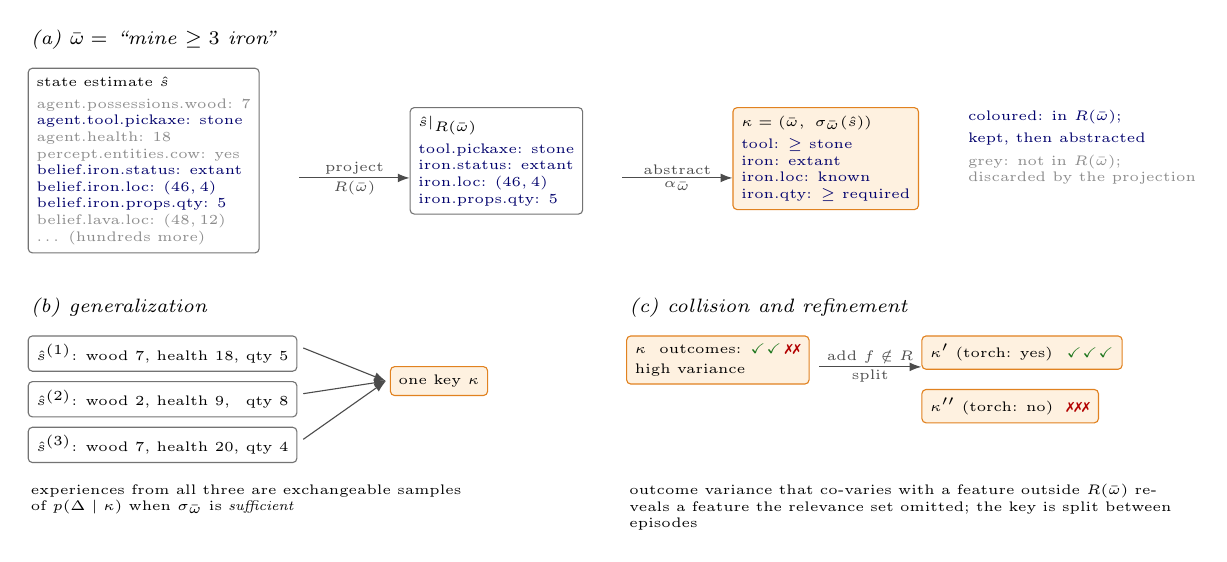
\begin{tikzpicture}[
  font=\small,
  rec/.style={draw=black!55, fill=white, rounded corners=1.5pt, inner sep=3pt, font=\tiny, align=left},
  key/.style={draw=BurntOrange!90!black, fill=BurntOrange!10, rounded corners=1.5pt, inner sep=3pt, font=\tiny, align=left},
  ar/.style={-{Latex[length=1.5mm]}, black!70, thin},
  pcap/.style={font=\scriptsize\itshape, inner sep=1pt},
  tlab/.style={font=\tiny, inner sep=1pt, align=center},
]

% ================= (a) construction =================
\node[pcap, anchor=west] at (0,4.75) {(a) $\bar\omega =$ ``mine $\ge 3$ iron''};

\node[rec, anchor=north west] at (0,4.4)
 {state estimate $\shat$\\[2pt]
  \textcolor{black!45}{agent.possessions.wood: 7}\\
  {\color{NavyBlue!85!black}agent.tool.pickaxe: stone}\\
  \textcolor{black!45}{agent.health: 18}\\
  \textcolor{black!45}{percept.entities.cow: yes}\\
  {\color{NavyBlue!85!black}belief.iron.status: extant}\\
  {\color{NavyBlue!85!black}belief.iron.loc: $(46,4)$}\\
  {\color{NavyBlue!85!black}belief.iron.props.qty: 5}\\
  \textcolor{black!45}{belief.lava.loc: $(48,12)$}\\
  \textcolor{black!45}{\dots\ (hundreds more)}};

\draw[ar] (3.45,3.0) -- node[tlab, above]{project} node[tlab, below]{$\Rel(\bar\omega)$} (4.85,3.0);

\node[rec, anchor=north west] at (4.85,3.9)
 {$\shat|_{\Rel(\bar\omega)}$\\[2pt]
  {\color{NavyBlue!85!black}tool.pickaxe: stone}\\
  {\color{NavyBlue!85!black}iron.status: extant}\\
  {\color{NavyBlue!85!black}iron.loc: $(46,4)$}\\
  {\color{NavyBlue!85!black}iron.props.qty: 5}};

\draw[ar] (7.55,3.0) -- node[tlab, above]{abstract} node[tlab, below]{$\alpha_{\bar\omega}$} (8.95,3.0);

\node[key, anchor=north west] at (8.95,3.9)
 {$\kappa=(\bar\omega,\ \sigma_{\bar\omega}(\shat))$\\[2pt]
  {\color{NavyBlue!85!black}tool: $\ge$ stone}\\
  {\color{NavyBlue!85!black}iron: extant}\\
  {\color{NavyBlue!85!black}iron.loc: known}\\
  {\color{NavyBlue!85!black}iron.qty: $\ge$ required}};

\node[tlab, anchor=north west, align=left] at (11.9,3.9)
 {{\color{NavyBlue!85!black}coloured: in $\Rel(\bar\omega)$;}\\[2pt]
  {\color{NavyBlue!85!black}kept, then abstracted}\\[2pt]
  \textcolor{black!45}{grey: not in $\Rel(\bar\omega)$;}\\
  \textcolor{black!45}{discarded by the projection}};

% ================= (b) many-to-one =================
\node[pcap, anchor=west] at (0,1.35) {(b) generalization};
\node[rec, anchor=north west, font=\tiny] at (0,1.0) {$\shat^{(1)}$: wood 7, health 18, qty 5};
\node[rec, anchor=north west, font=\tiny] at (0,0.42) {$\shat^{(2)}$: wood 2, health 9,\phantom{0} qty 8};
\node[rec, anchor=north west, font=\tiny] at (0,-0.16) {$\shat^{(3)}$: wood 7, health 20, qty 4};
\node[key, anchor=west] at (4.6,0.42) {one key $\kappa$};
\foreach \y in {0.84,0.26,-0.32}{ \draw[ar] (3.5,\y) -- (4.55,0.42); }
\node[tlab, anchor=north west, align=left, text width=5.6cm] at (0,-0.85)
 {experiences from all three are exchangeable samples of $p(\Delta\mid\kappa)$ when $\sigma_{\bar\omega}$ is \emph{sufficient}};

% ================= (c) refinement =================
\node[pcap, anchor=west] at (7.6,1.35) {(c) collision and refinement};
\node[key, anchor=north west] at (7.6,1.0) {$\kappa$\ \ outcomes: \textcolor{ForestGreen!85!black}{\checkmark\checkmark}\,\textcolor{Red!70!black}{\ding{55}\ding{55}}\\[1pt] high variance};
\draw[ar] (10.05,0.6) -- node[tlab, above]{add $f\notin\Rel$}node[tlab, below]{split} (11.35,0.6);
\node[key, anchor=north west] at (11.35,1.0) {$\kappa'$ (torch: yes)\ \ \textcolor{ForestGreen!85!black}{\checkmark\checkmark\checkmark}};
\node[key, anchor=north west] at (11.35,0.32) {$\kappa''$ (torch: no)\ \ \textcolor{Red!70!black}{\ding{55}\ding{55}\ding{55}}};
\node[tlab, anchor=north west, align=left, text width=6.9cm] at (7.6,-0.85)
 {outcome variance that co-varies with a feature outside $\Rel(\bar\omega)$ reveals a feature the relevance set omitted; the key is split between episodes};
\end{tikzpicture}

\caption{Signatures. (a) The signature of a state with respect to a canonical option is a projection onto the option's relevance set followed by a value abstraction; the great majority of the state is discarded, and quantities, tiers, and locators are replaced by the equivalence classes that matter for this option. (b) Because the projection is small and the abstraction coarse, many distinct states map to one key, and their experiences may be aggregated whenever the signature is sufficient in the sense of (\ref{eq:sufficient}). (c) When it is not, the omission shows up as outcome variance at a single key that co-varies with a feature outside the relevance set; consolidation adds that feature and splits the key.}
\label{fig:signature}
\end{figure}


Experience from one state is useful in another only if the two states agree on whatever determines the outcome of the option in question. A signature makes this equivalence explicit.

\paragraph{Canonical options.}
Options are natural-language strings, and semantically equivalent strings must map to a common key. A canonicalization module $\bar\omega=\mathrm{canon}(\omega)\sim\llm{canon}(\cdot\mid\omega,\{\bar\omega'\})$ maps an option to an existing canonical form from the set $\{\bar\omega'\}$ already in the store, or to a new normalized form if none matches. Parameters are folded into the canonical form (``gather $\ge 8$ logs'' rather than ``gather logs'' with the quantity elsewhere), so that the abstraction defined below can be fixed per canonical option. The mapping is cached, and all downstream keys use $\bar\omega$.

\paragraph{Relevance set and value abstraction.}
Each canonical option carries a \emph{schema} $(\Rel(\bar\omega),\alpha_{\bar\omega})$ consisting of
\begin{itemize}[leftmargin=1.5em,itemsep=1pt]
\item a \emph{relevance set} $\Rel(\bar\omega)=\Rel_{\mathrm{pre}}(\bar\omega)\cup\Rel_{\mathrm{eff}}(\bar\omega)\subseteq\calF$, where $\Rel_{\mathrm{pre}}$ contains the features that condition whether the option can be executed (required possessions, required tool tier, the status and locator of the element it refers to) and $\Rel_{\mathrm{eff}}$ the features that modulate its effect (the quantity available at the element, the agent's carrying capacity); and
\item a \emph{value abstraction} $\alpha_{\bar\omega}$ that maps the raw value of each feature in $\Rel(\bar\omega)$ to an equivalence class: quantities to threshold buckets relative to the option's requirement, tool-like attributes to tiers, locators to $\{\mathrm{known},\mathrm{unknown}\}$, belief status to $\{\mathrm{extant},\mathrm{consumed},\mathrm{unknown}\}$.
\end{itemize}
The schema is produced once, when the canonical option is first encountered, by a prompting module $\llm{schema}(\cdot\mid\bar\omega,\calF)$, and cached; it is never re-derived at write or read time, which guarantees that the same option yields the same key structure throughout the episode sequence. It is revised only by the refinement step below, between episodes.

\paragraph{Signature and key.}
The signature of a state estimate with respect to a canonical option is the abstracted projection
\begin{equation}
\sigma_{\bar\omega}(\shat)=\alpha_{\bar\omega}\big(\shat|_{\Rel(\bar\omega)}\big),
\label{eq:signature}
\end{equation}
and the \emph{experience key} is the pair
\begin{equation}
\kappa=(\bar\omega,\sigma_{\bar\omega}(\shat)),
\label{eq:key}
\end{equation}
serialized in a canonical feature order so that it is hashable. Since $\Rel(\bar\omega)$ is a small subset of $\calF$ and $\alpha_{\bar\omega}$ is coarse, many distinct states share a key, which is what allows experience to transfer (Figure~\ref{fig:signature}a,b).

\paragraph{Sufficiency and minimality.}
Let $\Delta$ denote the option-level state change observed when $\bar\omega$ is executed from $\shat$. The signature is \emph{sufficient} for $\bar\omega$ if
\begin{equation}
p(\Delta\mid\shat,\bar\omega)=p(\Delta\mid\sigma_{\bar\omega}(\shat),\bar\omega),
\label{eq:sufficient}
\end{equation}
i.e., the full state carries no information about the outcome beyond the signature, and \emph{minimal} if no strictly coarser relevance set or abstraction is sufficient. Sufficiency makes experiences stored under a common key exchangeable samples of one transition distribution, which is the condition under which their aggregation is meaningful; minimality maximizes the number of states that share a key. Neither property can be verified directly, but each has an observable proxy used below.

\paragraph{Schema refinement.}
An LLM-produced schema may omit a relevant feature. The omission manifests as a \emph{collision}: experiences stored under one key exhibit outcome variance that is explained by a feature outside $\Rel(\bar\omega)$. Between episodes, for each key whose outcome variance exceeds a threshold, the consolidation step searches the stored (unabstracted) start states for a feature $f\notin\Rel(\bar\omega)$ whose value co-varies with the outcome; if one is found, $f$ is added to $\Rel(\bar\omega)$, an abstraction for it is requested from $\llm{schema}$, and the key is split. Conversely, two keys differing in one feature whose outcome distributions are statistically indistinguishable are merged by coarsening $\alpha_{\bar\omega}$ on that feature. Refinement moves the schema toward sufficiency and merging toward minimality, using only the agent's own experience (Figure~\ref{fig:signature}c). When a schema changes, the experiences stored under the affected keys are re-keyed from their retained start states.

\paragraph{Distance between keys.}
For retrieval of near matches, the distance between two keys with the same canonical option is the weighted count of disagreeing signature features,
\begin{equation}
\dist(\kappa,\kappa')=\textstyle\sum_{f\in\Rel(\bar\omega)}w_f\,\mathbb{1}[\sigma_{\bar\omega}(\shat)_f\ne\sigma_{\bar\omega}(\shat')_f],
\qquad w_f=\begin{cases}w_{\mathrm{pre}} & f\in\Rel_{\mathrm{pre}}(\bar\omega)\\ w_{\mathrm{eff}} & \text{otherwise},\end{cases}
\label{eq:key-dist}
\end{equation}
with $w_{\mathrm{pre}}>w_{\mathrm{eff}}$, so that a near match that disagrees on a precondition is ranked below one that disagrees on an effect determinant. Keys with different canonical options are at infinite distance. Let $\mathrm{NN}_m(\kappa)$ denote the $m$ stored experiences with keys nearest to $\kappa$.

\paragraph{Granularities.}
The projection in (\ref{eq:signature}) is applied at three granularities, differing only in the relevance set: the \emph{option} signature $\Rel(\bar\omega)$ used for keys; the \emph{plan-tail} signature $\Rel(\omega_{i+1:n})$ used by the replanning monitor (\ref{eq:monitor}), which is the union over the remaining options; and the \emph{task} signature $\Rel(g)$, the union over the options expanded in the search tree, used as the state-equivalence key for reusing cached tree expansions across iterations and across episodes.

\subsection{Memory unit and store}
\label{sec:type2-unit}

\paragraph{Option experiences.}
The atomic unit is an \emph{option experience}, one per executed option,
\begin{equation}
x=\big(\kappa,\;\shat|_{\Rel(\bar\omega)},\;\hat\Delta,\;\hat\phi,\;\hat r,\;\Delta,\;\mathrm{outcome},\;\pi^{\ast},\;\prov,\;\mathrm{flag}\big),
\label{eq:experience}
\end{equation}
where $\kappa$ is the key at the option's start; the second entry is the unabstracted start state on the relevance set, retained for re-keying when a schema changes; $\hat\Delta$, $\hat\phi$, and $\hat r$ are the transition, feasibility verdict, and reward that the dynamics, feasibility, and reward modules produced for this option at planning time (from $\mathrm{pred}_i$ of the trace); $\Delta$ is the observed transition, the difference between $\shat_{t_{i-1}}$ and $\shat_{t_i}$ over all three state components, and therefore including every belief change of the option, among them the status changes to \emph{unknown} produced by the absence rule; $\mathrm{outcome}$ is copied from the trace; $\pi^\ast$ is the in-option code of the final, terminating attempt, together with the error messages of the failed attempts; $\prov$ records the episode index, the option index, and the replanning trigger, if any; and $\mathrm{flag}$ records whether the episode containing the option succeeded. An experience is a labeled example for each module: $(\kappa,\hat\Delta,\Delta)$ for the dynamics predictor, $(\kappa,\hat\phi,\mathrm{outcome})$ for the feasibility module, $(\kappa,\hat r,\mathrm{outcome})$ for the reward predictor, and $(\kappa,\pi^\ast)$ for code synthesis.

Options that were proposed and judged infeasible during planning, and options whose execution failed, are recorded with the same structure (with $\Delta$, $\pi^\ast$ empty where applicable). Negative experiences are what correct the option generator; a store restricted to successes would only reinforce it.

\begin{lifecycle}
$\kappa$ & option termination, from the schema of $\bar\omega$ & recomputed from the retained start state when the schema is refined or merged \\
$\shat|_{\Rel(\bar\omega)}$, $\hat\Delta$, $\hat\phi$, $\hat r$, $\Delta$, $\mathrm{outcome}$, $\pi^\ast$, $\prov$ & option termination, from the closed trace & none \\
$\mathrm{flag}$ & option termination (unset) & set at episode end from the episode outcome \\
\end{lifecycle}

\paragraph{Summaries.}
Experiences are the only record of what happened; everything else in the store is a summary maintained over them. Two summaries suffice, one per index under which experiences are looked up:
\begin{itemize}[leftmargin=1.5em,itemsep=1pt]
\item \emph{Per-key summary} $S(\kappa)$, for each experience key: the count $n(\kappa)$, the empirical success rate, an aggregate observed transition $\bar\Delta(\kappa)$ (feature-wise mode for discrete features, median for quantities), the variance of $\Delta$, and the verified code $\pi^\ast(\kappa)$, taken from the terminating attempt that has since required the fewest refinements. This is where environment stochasticity is handled: a single failure of ``find a creature of type $c$'' is an observation, five failures in six executions is a rate.
\item \emph{Per-type summary} $S(\type)$, for each element type: an empirical persistence distribution, obtained from the status changes to \emph{unknown} recorded in the $\Delta$ fields together with the elapsed time since $\tobs$; and a relevance flag. These are the two quantities Type 1 memory reads, the first at belief creation to set $\vol$ and the second at consolidation to prune (Section~\ref{sec:type1-type2}).
\end{itemize}
Both are aggregates of $\{x\}$ and could in principle be recomputed on demand; they are stored because they are read at every node expansion of the search, and recomputation would be linear in the number of experiences at the key.

\paragraph{Rules.}
The one component that is not an aggregate is the set of \emph{semantic rules} $\calK$, statements that generalize across keys rather than summarizing one: preconditions (``$\bar\omega$ requires $f=v$''), effects (``$\bar\omega$ yields $\Delta$ under $\sigma$''), and world regularities (``elements of type $c$ are found in regions of type $c'$''). Each rule carries a support count and the keys it was distilled from. Rules stand to experiences as Type 1's region beliefs stand to observations: both are produced by an LLM consolidation step, and neither is recoverable by aggregation.

\paragraph{Store.}
The store is therefore
\begin{equation}
\calX=\big(\{x\},\;S(\cdot),\;\calK\big),
\label{eq:store2}
\end{equation}
with $\{x\}$ indexed by key and by (episode, option index), and $S(\cdot)$ standing for the two families of summaries above. Quantities that a plan-level reader might expect to find as separate objects are views on this store rather than components of it: the option sequence executed in episode $k$ is the experiences with that episode index ordered by option index; the sequence of a successful episode, which the option generator uses as a template, is the same view restricted to $\mathrm{flag}=\mathrm{success}$; the replanning events of an episode are the triggers in their $\prov$ fields; and the record of belief invalidations, from which persistence is estimated, is a projection of the $\Delta$ fields. None of them is written separately.

\paragraph{Two histories.}
Unlike Type 1, which retains no observation history because a recursive filter suffices for its consumers, Type 2 retains $\{x\}$. The asymmetry is deliberate: Type 2's consumers need individual precedents rather than a current estimate. Nearest-neighbour retrieval (\ref{eq:key-dist}) returns particular experiences, and re-keying after a schema split requires each experience's unabstracted start state. Neither is recoverable from an aggregate, so the raw set is kept, bounded by the reservoir of Section~\ref{sec:type2-ops}.

\subsection{Operations}
\label{sec:type2-ops}
\begin{figure}[t]
\centering
% Experience memory over the episode sequence: write cadences and what crosses the boundary.
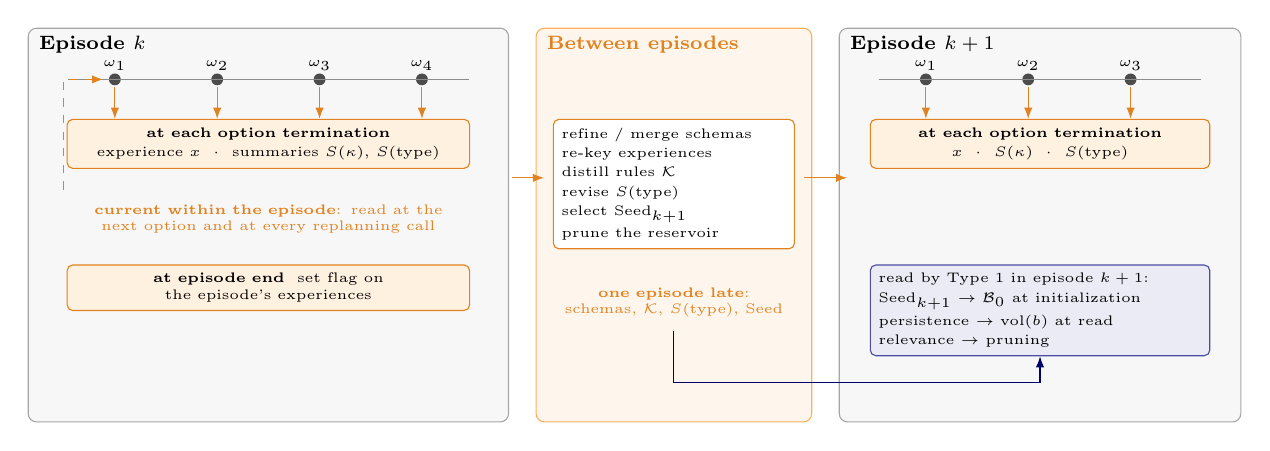
\begin{tikzpicture}[
  font=\small,
  zone/.style={rounded corners=3pt, draw=black!35},
  zlab/.style={font=\scriptsize\bfseries, anchor=north west, inner sep=2pt},
  wbox/.style={draw=BurntOrange!90!black, fill=BurntOrange!10, rounded corners=2pt, inner sep=3pt, font=\tiny, align=center},
  cbox/.style={draw=BurntOrange!90!black, fill=white, rounded corners=2pt, inner sep=3pt, font=\tiny, align=left},
  t1box/.style={draw=NavyBlue!70, fill=NavyBlue!8, rounded corners=2pt, inner sep=3pt, font=\tiny, align=left},
  tick/.style={circle, fill=black!70, inner sep=0pt, minimum size=1.5mm},
  ar/.style={-{Latex[length=1.4mm]}, BurntOrange!90!black, thin},
  arb/.style={-{Latex[length=1.4mm]}, black!60, thin},
  arr/.style={-{Latex[length=1.4mm]}, BurntOrange!90!black, thin, dashed},
  ar1/.style={-{Latex[length=1.4mm]}, NavyBlue!85!black, thin},
  tlab/.style={font=\tiny, inner sep=1pt, align=center},
]

% ================= zones =================
\fill[black!3, rounded corners=3pt] (0,0.2) rectangle (6.1,5.2);
\draw[zone] (0,0.2) rectangle (6.1,5.2);
\node[zlab] at (0.06,5.18) {Episode $k$};

\fill[BurntOrange!6, rounded corners=3pt] (6.45,0.2) rectangle (9.95,5.2);
\draw[zone, draw=BurntOrange!60] (6.45,0.2) rectangle (9.95,5.2);
\node[zlab, BurntOrange!90!black] at (6.51,5.18) {Between episodes};

\fill[black!3, rounded corners=3pt] (10.3,0.2) rectangle (15.4,5.2);
\draw[zone] (10.3,0.2) rectangle (15.4,5.2);
\node[zlab] at (10.36,5.18) {Episode $k+1$};

% ================= option terminations =================
\foreach \x/\i in {1.1/1, 2.4/2, 3.7/3, 5.0/4}{
  \node[tick] at (\x,4.55) {}; \node[font=\tiny, above, inner sep=1pt] at (\x,4.62) {$\omega_{\i}$};
  \draw[ar] (\x,4.45) -- (\x,4.05);
}
\foreach \x/\i in {11.4/1, 12.7/2, 14.0/3}{
  \node[tick] at (\x,4.55) {}; \node[font=\tiny, above, inner sep=1pt] at (\x,4.62) {$\omega_{\i}$};
  \draw[ar] (\x,4.45) -- (\x,4.05);
}
\draw[black!45] (0.5,4.55) -- (5.6,4.55);
\draw[black!45] (10.8,4.55) -- (14.9,4.55);

% ================= write at option termination =================
\node[wbox, text width=4.9cm, anchor=north] at (3.05,4.05)
  {\textbf{at each option termination}\\[1pt] experience $x$\ \ $\cdot$\ \ summaries $S(\kappa)$, $S(\mathrm{type})$};
\node[wbox, text width=4.1cm, anchor=north] at (12.85,4.05)
  {\textbf{at each option termination}\\[1pt] $x$\ \ $\cdot$\ \ $S(\kappa)$\ \ $\cdot$\ \ $S(\mathrm{type})$};

% read-back arrow inside the episode
\draw[arr] (0.45,3.15) -- (0.45,4.55) -- (0.95,4.55);
\node[tlab, anchor=north, BurntOrange!90!black, text width=5.4cm] at (3.05,3.0)
  {\textbf{current within the episode}: read at the next option and at every replanning call};

% ================= episode end =================
\node[wbox, text width=4.9cm, anchor=north] at (3.05,2.2)
  {\textbf{at episode end}\ \ set flag on the episode's experiences};

% ================= consolidation =================
\node[cbox, text width=2.85cm, anchor=north] at (8.2,4.05)
  {refine / merge schemas\\[1pt] re-key experiences\\[1pt] distill rules $\calK$\\[1pt] revise $S(\mathrm{type})$\\[1pt] select $\mathrm{Seed}_{k+1}$\\[1pt] prune the reservoir};
\draw[ar] (6.15,3.3) -- (6.55,3.3);
\draw[ar] (9.85,3.3) -- (10.4,3.3);
\node[tlab, anchor=north, BurntOrange!90!black, text width=3.0cm] at (8.2,1.95)
  {\textbf{one episode late}:\\ schemas, $\calK$, $S(\mathrm{type})$, $\mathrm{Seed}$};

% ================= into Type 1 of the next episode =================
\node[t1box, text width=4.1cm, anchor=north] (t1r) at (12.85,2.2)
  {read by Type 1 in episode $k+1$:\\[1pt]
   $\mathrm{Seed}_{k+1}\to\calB_0$ at initialization\\[1pt]
   persistence $\to\vol(b)$ at read\\[1pt]
   relevance $\to$ pruning};
\draw[ar1] (8.2,1.35) -- (8.2,0.7) -- (12.85,0.7) -- (t1r.south);
\end{tikzpicture}

\caption{The experience memory over the episode sequence. Objects written at option termination---the experiences and the summaries $S(\cdot)$---are current within the episode that wrote them, so they are read by the next option and by every replanning call of the same episode. What consolidation produces---the refined schemas, the rules $\calK$, and the revisions of $S(\type)$ and of the seed set that Type 1 memory reads---becomes available one episode later. The episode boundary is therefore the only point at which the schema of a key changes, and the only channel through which the state memory of a new episode is seeded.}
\label{fig:lifecycle}
\end{figure}

\paragraph{Initialization.}
Before episode 1 the store is empty, with two exceptions. The verified-code field of $S(\kappa)$ may be seeded with an existing library of control programs if one is available for the environment; each seeded program is entered under a key derived from its documented preconditions. And $S(\type)$ is populated lazily: the first time an element type is encountered, its persistence class is assigned by prompting an LLM with the type, and its relevance flag is set. The LLM is the prior for everything else, and the store exists to correct that prior; seeding the store from the LLM would be circular.

\paragraph{Write.}
Writes occur at three cadences, summarized in the table below and, over the episode sequence, in Figure~\ref{fig:lifecycle}.
\begin{enumerate}[leftmargin=1.5em,itemsep=1pt]
\item \emph{Option termination.} The experience $x$ is assembled from the closed trace. The canonical option and schema are looked up (created on first encounter), the key is computed, and $S(\kappa)$ is updated online, including its verified-code field if the final attempt terminated the option. The persistence statistics in $S(\type)$ are updated from the belief status changes carried by $\Delta$.
\item \emph{Episode end.} The $\mathrm{flag}$ of the episode's experiences is set from the outcome. Nothing else is written: the episode record and the plan library are views (\ref{eq:store2}).
\item \emph{Between episodes.} Consolidation runs offline: (i) schema refinement and merging (Section~\ref{sec:signature}), followed by re-keying of the affected experiences and recomputation of their $S(\kappa)$; (ii) rule distillation, $\calK\leftarrow\llm{consolidate}(\cdot\mid\calK,C)$, applied to clusters $C$ of experiences grouped by canonical option, with priority to clusters containing failures or large prediction divergence $\|\hat\Delta-\Delta\|$, since these are where the prior is wrong; (iii) revision of the persistence and relevance fields of $S(\type)$, and selection of the seed set $\mathrm{Seed}_{k+1}$ (both in Section~\ref{sec:type1-type2}); (iv) bounding of $\{x\}$ by retaining, per key, a fixed-size reservoir plus every experience referenced by a rule.
\end{enumerate}

\begin{center}\small
\begin{tabular}{@{}>{\raggedright\arraybackslash}p{0.24\textwidth}>{\raggedright\arraybackslash}p{0.22\textwidth}>{\raggedright\arraybackslash}p{0.18\textwidth}>{\raggedright\arraybackslash}p{0.28\textwidth}@{}}
\toprule
Object & Option termination & Episode end & Between episodes \\
\midrule
Canonical options, schemas & created on first encounter & --- & refined, merged \\
Experiences $\{x\}$ & created & $\mathrm{flag}$ set & re-keyed; reservoir pruned \\
Per-key summary $S(\kappa)$ & updated & --- & recomputed for split or merged keys \\
Per-type summary $S(\type)$ & persistence statistics updated & --- & persistence and relevance revised \\
Rules $\calK$ & --- & --- & distilled \\
Seed set $\mathrm{Seed}_{k+1}$ & --- & --- & selected from the terminal beliefs \\
\bottomrule
\end{tabular}
\end{center}

\paragraph{Read.}
A read for key $\kappa$ returns
\begin{equation}
\Read(\calX,\kappa)=\big(S(\kappa),\;\mathrm{NN}_m(\kappa),\;\calK(\kappa)\big),
\label{eq:type2-read}
\end{equation}
the exact-match summary including its verified code, the $m$ nearest experiences under (\ref{eq:key-dist}), and the rules whose antecedents mention $\bar\omega$ or a feature in $\Rel(\bar\omega)$. A read at the planner root additionally returns the successful-episode view of $\{x\}$. Each module receives the parts of the read view relevant to it; as with Type 1, the store is never placed in a prompt.

\paragraph{Precedence.}
The rule that decides between the LLM prior and stored experience is the mechanism by which the system improves without gradient updates, and is stated once for all modules. By default, precedence is \emph{soft}: the read view enters the module's prompt as evidence and the module's output remains a sample from the LLM. For the dynamics and feasibility modules, precedence becomes \emph{hard} when the exact-match count is sufficient, $n(\kappa)\ge n_0$: the module's output is replaced by the empirical aggregate, and the LLM is not called. The threshold $n_0$ trades the LLM's generalization against the store's specificity and is the single parameter that interpolates between a prompting-only system ($n_0=\infty$) and a tabular one ($n_0=1$).

\paragraph{Order of operations at option termination.}
Both memories are written, and the replanning monitor is run, at the termination of every option, in the following fixed order: consolidation (\ref{eq:consol}) is applied to the belief set; the trace is closed on the consolidated estimate; the Type 2 write of the option-termination cadence is applied (the experience is created and the summaries are updated); the monitor (\ref{eq:monitor}) is evaluated; and, if a trigger fires, the planner is invoked. Consequently a replanning call at $t_i$ reads the experiences of options $1,\dots,i$ of the current episode, including the experience of the option whose termination triggered it. This is the case that matters most: the plan-invalidation trigger fires because the prior was wrong about $\omega_i$, and the experience of $\omega_i$ records the divergence $(\hat\Delta_i,\Delta_i)$; the replanner's dynamics module retrieves it as the nearest neighbour at the same key and does not repeat the error.

\paragraph{Availability within an episode.}
The objects written at option termination---the raw experiences, hence $\mathrm{NN}_m$, and the summaries $S(\cdot)$---are current within the episode in which they were written. The rules $\calK$, the revisions of $S(\type)$, the seed set, and the schema refinements are produced by consolidation and become available one episode late. In-episode improvement therefore flows through nearest-neighbour evidence, empirical summaries, and verified code; in particular, hard precedence rarely fires within the first episodes, since the counts $n(\kappa)$ are small, and early improvement is entirely through soft precedence. Experiences of the current episode have $\mathrm{flag}$ unset, so they inform the dynamics, feasibility, reward, and code modules but do not yet contribute to $\Omega^{+}$, $\Omega^{-}$, or the successful-episode view.

\subsection{Interaction with planning and execution}
\label{sec:type2-interaction}

Each module of Section~\ref{sec:type1-plan} becomes retrieval-augmented; the conditioning is extended and the prompt template is amended to describe the retrieved evidence. Writing $\kappa$ for the key of the state and option under consideration:
\begin{itemize}[leftmargin=1.5em,itemsep=1pt]
\item \emph{Option generator.} $\llm{propose}(\cdot\mid\tau_{i-1},\Omega^{+},\Omega^{-},\Lambda)$, where $\Omega^{+}$ and $\Omega^{-}$ are the sets of canonical options with high and with repeatedly low empirical success in $S(\kappa)$ under $\sigma_{\bar\omega}(\shat_{i-1})$, and $\Lambda$ is the successful-episode view of $\{x\}$: options that have succeeded from the current state are offered as candidates, options with repeated failure are listed as candidates to avoid, and the sequences in $\Lambda$ are offered as templates. The feasibility module receives $S(\kappa)$ and $\calK(\kappa)$ and, under hard precedence, returns the empirical verdict.
\item \emph{Dynamics predictor.} $\llm{dyn}(\cdot\mid\shat_{i-1},\omega,\mathrm{NN}_m(\kappa),\calK(\kappa))$ under soft precedence; $\shat_i=\shat_{i-1}\oplus\bar\Delta(\kappa)$ under hard precedence, where $\oplus$ applies the aggregate delta. This is the direct remedy for compounding prediction error: along any segment of a rollout that passes through experienced keys, the predicted trajectory is anchored to observed transitions rather than extrapolated by the LLM.
\item \emph{Reward predictor.} The evaluation questions in (\ref{eq:reward}) receive the empirical success rate in $S(\kappa)$, so that options with a history of failing from states like the current one are debited accordingly.
\item \emph{Executor.} When $S(\kappa)$ carries verified code, that code is executed first; code synthesis is invoked only on a miss or on failure of the verified code, in which case the refinement loop proceeds from the verified code rather than from scratch.
\item \emph{Replanning monitor.} The monitor receives the variance of $\Delta$ recorded in $S(\kappa)$ at the keys of the plan tail. A high-variance option is a predicted source of divergence; the horizon-exhaustion trigger is advanced to fire before such an option rather than after, so that the search that follows it is performed from an observed rather than a predicted state.
\end{itemize}

\subsection{Interaction with Type 1 memory}
\label{sec:type1-type2}

The two memories exchange information through the objects listed in the write table of Section~\ref{sec:type2-ops}. In one direction, Type 1 supplies the observed transitions $\Delta$, computed from the state estimates the trace (\ref{eq:trace}) records at the option's start and termination; the belief status changes to \emph{unknown} produced by the absence rule travel inside $\Delta$, and are the raw material of the persistence estimate below. In the other direction, Type 1 reads the per-type summary $S(\type)$ and the seed set at three fixed points, which consolidation revises between episodes.

\begin{enumerate}[leftmargin=1.5em,itemsep=1pt]
\item \emph{Persistence}, read at belief creation to set $\vol$. Each element type accumulates, from the invalidation events in the $\Delta$ fields, an empirical distribution over the elapsed time between $\tobs$ and the status change to \emph{unknown}. Once a type has at least $n_V$ such events, the LLM-assigned persistence class in $S(\type)$ is replaced by a discount function derived from that distribution, and the read operation (\ref{eq:read}) applies the function in place of the class-based discount. Beliefs already in the seed set keep their $\vol$; beliefs created in the next episode take the revised entry.
\item \emph{Relevance}, read by the pruning step of consolidation (\ref{eq:consol}). Between episodes, once at least one episode has succeeded, the relevance flag in $S(\type)$ is set for the element types that appear in $\Rel_{\mathrm{pre}}$ of the canonical options of the successful-episode view, and cleared otherwise; beliefs about types without the flag are pruned at the next option termination, so the belief set stops growing with types that have never mattered for the goal. If no episode has succeeded, the flags are unchanged.
\item \emph{Seed set} $\mathrm{Seed}_{k+1}$, read at initialization (\ref{eq:init}). From the beliefs retained at the end of episode $k$ (observed, permanent, extant), a belief is admitted if its type has no invalidation event with elapsed time shorter than one episode; beliefs of types observed to become invalid within an episode are not carried over even if classed permanent. Admitted beliefs enter episode $k+1$ unchanged except that $\tobs$ retains the episode index $k$, which the read discount treats as maximally stale within the permanent class.
\end{enumerate}

Under this exchange, the only Type 1 fields whose values depend on Type 2 are $\vol$ (through the persistence field of $S(\type)$) and the initial contents of $\calB_0$ (through $\mathrm{Seed}_k$); the only Type 1 behaviour that depends on Type 2 is the pruning step of consolidation (through the relevance flag). All other Type 1 fields and operations are determined within the episode as specified in Section~\ref{sec:type1-est}.

\end{document}